




\documentclass{article}



\usepackage{amsmath}
\usepackage{amsfonts}
\usepackage{listings}

\usepackage[braket, qm]{qcircuit}
\usepackage{graphicx}





\title{Quantum Computing for Engineers}
\author{Osama Muhammad Raisuddin}







\begin{document}

\maketitle

\tableofcontents


  \vspace{10pt}
    \hrule
  \vspace{10pt}
This is the Abstract 
  \vspace{10pt}








\section{Introduction}


Quantum computing is an emerging area of research with great potential for engineering and scientific computing applications. Endowed with quantum mechanical properties such as superposition, entanglement and tunneling, quantum computers can enable exponential speedups over classical computers for some problems. The advantage can be realized in both time and energy consumption. 

All classical computation can be performed on quantum computers using reversible versions of logic gates. However, this approach is inefficient and required large overheads. To take advantage of quantum computers new algorithms have been developed and are an active area of research. Due to stark differences with classical computation, the engineering community has limited exposure to quantum computing and quantum algorithms. 

In this review we aim to provide an introduction to quantum computing with demonstration of concepts and ideas with code. Quantum algorithms relevant to engineers are presented in detail with implementation.





%\section{Quantum Information}
%
%\subsection{Quantum States}
%
%\subsection{Operators}
%
%\subsection{Measurements}
%
%\subsection{Composite Systems}
%
%\subsection{Density Operators}
%
%\subsection{Born Rule}









This section should give an introduction to the state spaces of the qubits, operators, the Kronecker products, and densoty operator representation. 

The Born Rule needs to be introduced. The no-cloning theorem can also be introduced here.



%\subsection{Postulates of Quantum Mechanics}
%
%\subsubsection{State Space}
%
%\subsubsection{Evolution}
%
%\subsubsection{Measurement}
%
%\subsubsection{Composite Systems}




\section{Quantum Computation}

In this section we abstract away details of quantum information and the underlying physics of a quantum computer and present the computational model for quantum computing. Since all gate-based quantum computers share the same computational model, this is a safe starting point for beginners. Implementation of quantum algorithms does not require knowledge beyond these fundamental elements.

\subsection{Qubits and Qudits}

A 'qubit', or a quantum bit, is the quantum analogue of a classical bit. It is the elementary information unit in quantum computing. A qubit is a two-dimensional quantum system with dimensions typically labelled '0' and'1' analogous to the states of a classical bit. A qubit is exists in the Hilbert space $ \mathcal{H} : \mathbb{C}^2$ and is represented in bra-ket (or Dirac) notation as:
\begin{equation}
\lvert \psi \rangle = \alpha \lvert 0 \rangle + \beta \lvert 1 \rangle
\end{equation}
where 
$ \lvert \alpha \rvert ^2 + \lvert \beta \rvert ^2 = 1$
 according to the Born rule and 
$ \lvert \psi \rangle \in \mathbb{C}^2$
 denotes the quantum state of the qubit. 
$ \lvert 0 \rangle$ and $ \lvert 1 \rangle $
 are the basis states in the 
$ 0-1$
 basis, corresponding to the basis vectors 
$ \lvert 0 \rangle = \begin{pmatrix}1 \\ 0\end{pmatrix} $
 and 
$ \lvert 1 \rangle = \begin{pmatrix}0 \\ 1\end{pmatrix} $
. 
$ \alpha $ and $ \beta $
 are the 'probability amplitudes' of the state 
$ \lvert \psi \rangle $
, corresponding to a probabilities of measuring the qubit $ \lvert \psi \rangle $ in states $ \lvert 0 \rangle $ and $ \lvert 1 \rangle $ with probailitities $ \lvert \alpha \rvert ^2 $ and $ \lvert \beta \rvert ^2 $ respectively. Note that once a measurement is performed on qubit $ \lvert \psi \rangle $ to obtain a measured state of either $ \lvert 0 \rangle $ or $ \lvert 1 \rangle $, the state $ \lvert \psi \rangle $ is destroyed and further measurements (without any other subsequent operations) will repeatedly yield the same state that was measured.

The state $ \lvert \psi \rangle $ is a 'ket'. The corresponding 'bra'  $\langle \psi \rvert$ is the adjoint, or the complex transpose of the 'ket'. As an example, the basis states form the kets
 $ \langle 0 \rvert =  \begin{pmatrix}
1 \; 0
\end{pmatrix} $
 and 
$\langle 1 \rvert =  \begin{pmatrix}
0 \; 1
\end{pmatrix} $.

A qudit is higher-dimensional generalization of of a qubit, s.t. $ \lvert \psi \rangle \in \mathbb{C}^d , \, d>2$.



\subsection{Registers of Qubits}

A register of qubits is a collection of $ n $ qubits, whose combined state is represented as the quantum system $ \lvert \psi \rangle \in  \mathbb{C}^{2^{n}}$, corresponding to a tensor product of the individual Hilbert spaces of the qubits.  The combined state $ \lvert \psi  \rangle $ of two individual qubits $ \lvert \psi _ 0 \rangle = \alpha_1 \lvert 0 \rangle + \beta_1 \lvert 1 \rangle $ and $ \lvert \psi _ 1 \rangle = \alpha_2 \lvert 0 \rangle + \beta_2 \lvert 1 \rangle $ may be represented in Dirac notation as a Kronecker product of the individual qubits with various equivalent notations:

\begin{multline}
\lvert \psi \rangle = \lvert \psi _ 1 \rangle \otimes \lvert \psi _ 2 \rangle 
= \lvert \psi _ 1 \rangle \lvert \psi _ 2 \rangle
= \lvert \psi _ 1 \psi _ 2 \rangle
\\
= (\alpha_1 \lvert 0 \rangle      + \beta_1 \lvert 1 \rangle)(\alpha_2 \lvert 0 \rangle      + \beta_2 \lvert 1 \rangle)
\\
= \alpha_1 \alpha_2 \lvert 0 \rangle \lvert 0 \rangle         
+ \alpha_1 \beta_2 \lvert 0 \rangle \lvert 1 \rangle      
+ \alpha_2 \beta_1 \lvert 1 \rangle\lvert 0 \rangle        
+ \beta_1 \beta_2 \lvert 1 \rangle\lvert 1 \rangle
\\
= \alpha_1 \alpha_2 \lvert 0 \rangle \otimes \lvert 0 \rangle         
+ \alpha_1 \beta_2 \lvert 0 \rangle  \otimes \lvert 1 \rangle      
+ \alpha_2 \beta_1 \lvert 1 \rangle  \otimes \lvert 0 \rangle        
+ \beta_1 \beta_2 \lvert 1 \rangle  \otimes \lvert 1 \rangle
\\
= \alpha_1 \alpha_2 \lvert 0  0 \rangle 
+ \alpha_1 \beta_2 \lvert 0 1 \rangle 
+ \alpha_2 \beta_1 \lvert 1  0 \rangle 
+ \beta_1 \beta_2 \lvert 1 1 \rangle
\\
= \alpha_1 \alpha_2        \begin{pmatrix}1\\0\end{pmatrix} \otimes \begin{pmatrix}1\\0\end{pmatrix} 
+ \alpha_2 \beta_1           \begin{pmatrix}1\\0\end{pmatrix} \otimes \begin{pmatrix}0\\1\end{pmatrix} 
+ \alpha_1 \beta_2            \begin{pmatrix}0\\1\end{pmatrix} \otimes \begin{pmatrix}1\\0\end{pmatrix} 
+ \beta_1 \beta_2               \begin{pmatrix}0\\1\end{pmatrix} \otimes \begin{pmatrix}0\\1\end{pmatrix} 
\\
= \alpha_1 \alpha_2        \begin{pmatrix}1\\0\\0\\0\end{pmatrix} 
+ \alpha_2 \beta_1           \begin{pmatrix}0\\1\\0\\0\end{pmatrix} 
+ \alpha_1 \beta_2            \begin{pmatrix}0\\0\\1\\0\end{pmatrix} 
+ \beta_1 \beta_2               \begin{pmatrix}0\\0\\0\\1\end{pmatrix} 
= \begin{pmatrix} \alpha_1 \alpha_2 \\  \alpha_2 \beta_1  \\  \alpha_1 \beta_2 \\  \beta_1 \beta_2 \end{pmatrix} 
.
\end{multline}


Additonal qubits will follow the same pattern, resulting in an exponentially large state space for the qubits. Note that the ordering of qubits is arbitrary, and a change in ordering shuffles the representation of the state corresponding the Kronecker product; typically one may choose the most conventient order for their application.

%Here, we provide an example code in Qiskit to allocate a register of qubits:

%\lstinputlisting[language=Python]{code_snippets/qubit_register.py}






\subsection{Gates}

In the gate-based quantum computing model operations on qubits are represented as quantum gates, or simply gates. Some of the gates are analogous to classical gate operations. However, some quantum gates may not have a corresponding classical counterpart.

Gates can be conveniently represented as complex matrices, in line with the column vector representation of qubits. The most basic gates are single qubit gates represented as $\mathbb{C}^{2\times2}$. Some important single-qubit gates are  the Pauli gate set $\{I,X,Y,Z\}$ and the Hadamard gate $H$.

Gate can also act on multiple qubits, in which case they can be represented in $\mathbb{C}^{2^{n}\times2^{n}}$. Multiple qubit gates typically arise as controlled versions of gates, of which $CNOT$ is a commonly used one. The $SWAP$ gate is another common gate which swaps the states between qubits.

All quantum gates are unitary operations, which ensures normalization of quantum states in line with the Born rule. Consequantly, all quantum gates are also reversible operations, with the reverse operation simply being the Hermitian transpose or conjugate transpose of the quantum gate.

Gates acting on qubits are typically represented as left multiplication. As an example, consider a register of three qubits in the state $ \lvert 000 \rangle $. Applying a Hadamard gate to the first qubit (from the left) and a Pauli X gate to the last qubit is represented as:

\begin{equation}
(H\otimes I\otimes X) \lvert 000 \rangle = (H \otimes I \otimes I) \lvert 001 \rangle = \frac{1}{\sqrt{2}} (\lvert 001 \rangle + \lvert 101 \rangle)
\end{equation}

As another example, consider a  register of two qubits with a Hadamard gate applied to the first qubit and a CNOT gate controlled by the first qubit applied to the second qubit:

\begin{equation}
( \lvert 00 \rangle \langle 00 \rvert + 
\lvert 01 \rangle \langle 01 \rvert + 
\lvert 10 \rangle \langle 11 \rvert + 
\lvert 11 \rangle \langle 10 \rvert
 )(H \otimes I) \lvert 00 \rangle 
=
\lvert 00 \rangle + \lvert 11 \rangle 
\end{equation}

Note how the order of operations progresses from right to left. It is common practice not to include the $I$ gate when the qubits on which the operation is applied is implied.

Similar to classical Boolean logic, quantum gates can also form a universal gate set. This implies that any arbitrary quantum gate can be approximated using a universal gate set. The Solovay-Kitaev theorem is a central theorem in quantum computing which shows that the approximation error using a universal gate set scales as $ O (\log^c (\frac{1}{\epsilon}))$ for a single-qubit gate where $ c \approx 2$ and $O(m \log ^c (\frac{m}{\epsilon}))$ for a a set of $m$ $CNOT$s  and single-qubit unitaries. These correspond to a polylogarithmic increase in the original number of gates.

Underlying hardware implementations can have a variety of gate sets. Algorithms are typically agnostic to the hardware implementation, since the gates are converted to the target hardware's gate set in a process called transpilation.



\subsection{Measurement}

A quantum state is defined using probability amplitudes. In order to read a state a series of measurements of the state need to be performed, and the measurement statistics will correspond to the probability amplitudes of the quantum state.

In gate-based quantum computing projective measurements are typically used and are represented by a 'meter' symbol. The measurement operation is a projection onto the $ \lvert 0 \rangle $ $ \lvert 1 \rangle $ basis. As an example, consider a two-qubit system in the state $ \frac{1}{2} ( \lvert 00 \rangle + \lvert 01 \rangle + \lvert 10 \rangle + \lvert 11 \rangle )$, with a measurement being performed on the first qubit. If the first qubit is measured in the state $ \lvert 0 \rangle  $ , the final state is:
 \begin{equation}
( \rvert 0 \rangle \langle 0 \rvert \otimes I ) (\frac{1}{2} ( \lvert 00 \rangle + \lvert 01 \rangle + \lvert 10 \rangle + \lvert 11 \rangle ) )
=
\frac{1}{\sqrt{2}} (\lvert 00 \rangle + \lvert 01 \rangle )
\end{equation}

Similarly, if the first qubit is measured in the state $ \lvert 1 \rangle $ the final state is:

 \begin{equation}
( \rvert 1 \rangle \langle 1 \rvert \otimes I ) (\frac{1}{2} ( \lvert 00 \rangle + \lvert 01 \rangle + \lvert 10 \rangle + \lvert 11 \rangle ) )
=
\frac{1}{\sqrt{2}} (\lvert 10 \rangle + \lvert 11 \rangle )
\end{equation}


Measurements may be performed to either read out an entire quantum register or as a flag to indicate successful operation by measuring ancilla qubits.

Note that measurements will provide the squared moduli (amplitudes) of the complex numbers defining the probability amplitude of a quantum state. In order to recover additonal information, like the arguments (phases),  a process known as quantum state tomography [ref] is performed. Quantum states also have an overall phase. The overall phase is not measurable; only relative phase between two states is measurable.


%\subsubsection{Principle of Deferred Measurement}
%
%Measurement operations can usually be pushed forward till the end 

\subsection{Circuits}

Working with algebraic forms of algorithms can be unwieldy and difficult to visualize. Quantum circuits are a convenient representation of qubits and the operation sequence.





 As an example, consider a register of three qubits $\lvert A B C \rangle $, with an $H$ gate applied to the $A$ and an $X$ gate applied to $C$, followed by a $CNOT$ gate controlled by the $A$ applied to $B$, and finally measurements on all the qubits. These operations can conveniently be represented in circuit form as:



\begin{figure}[h]
\centering
\scalebox{1.0}{
\Qcircuit @C=1.0em @R=0.2em @!R { \\
	 	\nghost{A :  } & \lstick{A :  } & \gate{\mathrm{H}} & \ctrl{1} \barrier[0em]{2} & \qw & \meter & \qw & \qw & \qw & \qw\\
	 	\nghost{B :  } & \lstick{B :  } & \qw & \targ & \qw & \qw & \meter & \qw & \qw & \qw\\
	 	\nghost{C :  } & \lstick{C :  } & \gate{\mathrm{X}} & \qw & \qw & \qw & \qw & \meter & \qw & \qw\\
	 	\nghost{\mathrm{{Classical\;Bits} :  }} & \lstick{\mathrm{{Classical\;Bits} :  }} & \lstick{/_{_{3}}} \cw & \cw & \cw & \dstick{_{_{\hspace{0.0em}0}}} \cw \ar @{<=} [-3,0] & \dstick{_{_{\hspace{0.0em}1}}} \cw \ar @{<=} [-2,0] & \dstick{_{_{\hspace{0.0em}2}}} \cw \ar @{<=} [-1,0] & \cw & \cw\\
\\ }}

\caption{Circuit with gates and measurements.}
\label{fig:first_circuit}

\end{figure}


Note that the operations are ordered from left to right, unlike operations ordered right to left in algebraic notation. A controlled operation can be applied conditioned on the control qubit being either in the state $1$ or  $0$. This in indicated in a quantum circuit with a filled or empty circle respectively, as shown in Figure \ref{fig:gate_conditions}.

\begin{figure}[h]

\centering
\scalebox{1.0}{
\Qcircuit @C=1.0em @R=0.2em @!R { \\
	 	\nghost{A :  } & \lstick{A :  } & \ctrl{1} & \ctrlo{1} & \qw & \qw\\
	 	\nghost{B :  } & \lstick{B :  } & \targ & \targ & \qw & \qw\\
\\ }}

\caption{$CNOT$ gates conditioned on $A$ in states $0$ and $1$.}
\label{fig:gate_conditions}

\end{figure}



Quantum registers can be ordered using either little-endian or big-endian notation. Little-endian ordering corresponds to the right-most qubit in algeraic notation indexed as $0$ and big-endian corresponds to the left-most qubit indexed as $0$. Qiskit uses little-endian ordering.

As an example, we repeat the example in Figure \ref{fig:first_circuit} but with $\lvert ABC \rangle$ being denoted as $\lvert \psi \rangle$. Consistent with Qiskit, in little-endian notation $\lvert A\rangle$, $\lvert B\rangle$, and $\lvert C\rangle$ correspond to $\lvert \psi _2 \rangle$, $\lvert \psi _1 \rangle$, and $\lvert \psi _0 \rangle$. We provide an example code: starting with big-endian notation and converting to little-endian at the end.


\lstinputlisting[language=Python]{code_snippets/endian.py}




\begin{figure}[h]


\scalebox{1.0}{
\Qcircuit @C=1.0em @R=0.2em @!R { \\
	 	\nghost{{\psi}_{0} :  } & \lstick{{\psi}_{0} :  } & \gate{\mathrm{X}} & \qw \barrier[0em]{2} & \qw & \qw & \qw & \meter & \qw & \qw\\
	 	\nghost{{\psi}_{1} :  } & \lstick{{\psi}_{1} :  } & \qw & \targ & \qw & \qw & \meter & \qw & \qw & \qw\\
	 	\nghost{{\psi}_{2} :  } & \lstick{{\psi}_{2} :  } & \gate{\mathrm{H}} & \ctrl{-1} & \qw & \meter & \qw & \qw & \qw & \qw\\
	 	\nghost{\mathrm{{Classical\;Bits} :  }} & \lstick{\mathrm{{Classical\;Bits} :  }} & \lstick{/_{_{3}}} \cw & \cw & \cw & \dstick{_{_{\hspace{0.0em}0}}} \cw \ar @{<=} [-1,0] & \dstick{_{_{\hspace{0.0em}1}}} \cw \ar @{<=} [-2,0] & \dstick{_{_{\hspace{0.0em}2}}} \cw \ar @{<=} [-3,0] & \cw & \cw\\
\\ }}

\caption{Output of Example code}


\end{figure}




\subsection{Superposition}

Superposition is a central property of quantum computing. A quantum state can exist in a superposition of states. As an example, a single qubit $\lvert \psi \rangle$ can exist in a superposition of $\lvert 0 \rangle$ and $\lvert 1 \rangle$. A register of $n$ qubits can exist in an exponentially large superposition of $N=2^n$ states. The Hadamard gate puts qubits in superposition. As an example, we provide the following code to put qubits in uniform superposition and measure their states:

\begin{figure}[h]

\centering

\scalebox{1.0}{
\Qcircuit @C=1.0em @R=0.2em @!R { \\
	 	\nghost{{\psi}_{0} :  } & \lstick{{\psi}_{0} :  } & \gate{\mathrm{H}} & \meter & \qw & \qw & \qw & \qw\\
	 	\nghost{{\psi}_{1} :  } & \lstick{{\psi}_{1} :  } & \gate{\mathrm{H}} & \qw & \meter & \qw & \qw & \qw\\
	 	\nghost{{\psi}_{2} :  } & \lstick{{\psi}_{2} :  } & \gate{\mathrm{H}} & \qw & \qw & \meter & \qw & \qw\\
	 	\nghost{\mathrm{{Classical\;Bits} :  }} & \lstick{\mathrm{{Classical\;Bits} :  }} & \lstick{/_{_{3}}} \cw & \dstick{_{_{\hspace{0.0em}0}}} \cw \ar @{<=} [-3,0] & \dstick{_{_{\hspace{0.0em}1}}} \cw \ar @{<=} [-2,0] & \dstick{_{_{\hspace{0.0em}2}}} \cw \ar @{<=} [-1,0] & \cw & \cw\\
\\ }}

\caption{Circuit for uniform superposition.}

\end{figure}


\lstinputlisting[language=Python]{code_snippets/uniform_superposition.py}

\begin{figure}[h]
\centering

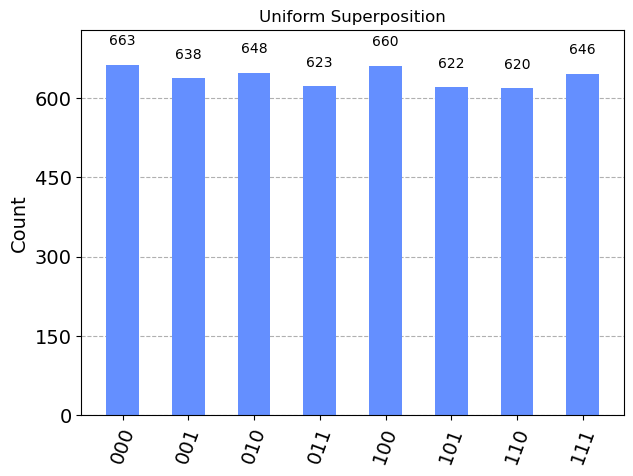
\includegraphics[scale=0.5]{code_snippets/uniform_superposition_output.png}


\caption{Output of Uniform Superposition code}

\end{figure}



\subsection{Entanglement}

Entanglement is another property unique to quantum computation. Entangled qubits have a correlated state. A maximal entanglement for a pair of qubits means that the full state of the one qubit can be determined completely by measuring the state of the second state. The simplest set of maximally entangled states are the Bell states:


 \begin{multline}
\lvert \Phi ^+ \rangle = \frac{1}{\sqrt{2}} ( \lvert 00 \rangle + \lvert 11 \rangle ), \lvert \Phi ^+ \rangle = \frac{1}{\sqrt{2}} ( \lvert 00 \rangle - \lvert 11 \rangle ), \\ \lvert \Psi ^+ \rangle = \frac{1}{\sqrt{2}} ( \lvert 01 \rangle + \lvert 10 \rangle ), \lvert \Psi ^+ \rangle = \frac{1}{\sqrt{2}} ( \lvert 01 \rangle - \lvert 10 \rangle ),
\end{multline}

As an example, if the first qubit of the state $ \lvert \Phi ^+ \rangle = \frac{1}{\sqrt{2}} ( \lvert 00 \rangle + \lvert 11 \rangle ) $ is measured as $0$, the second qubit is also in the state $0$, and if the first qubit is measured as $1$, the second qubit is also in the state $1$. Note that this is not the same as the state $ \lvert \psi \rangle = \lvert 00 \rangle $, which is not an entangled state.

Mathematically, entangled qubits cannot be separated into a Kronecker product. The state $ \lvert 00 \rangle $ can be written as $ \lvert 0 \rangle \otimes \lvert 0 \rangle $, however, it is impossible to separate $ \lvert \Psi^+ \rangle $ into such a Kronecker product.


Here, we provide an example of a circuit creating the entangled state $ \lvert \Phi^+ \rangle $:


\lstinputlisting[language=Python]{code_snippets/entanglement.py}



\begin{figure}[h]
\centering

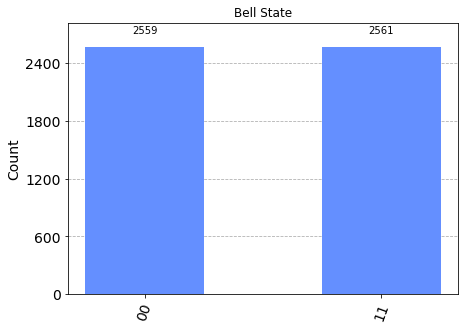
\includegraphics[scale=0.5]{code_snippets/entanglement_output.png}


\caption{Output of Entanglement code}

\end{figure}




\subsection{Reversible Computation}

All quantum gates are reversible, since they are unitary operations. Therefore, the corresponding inverse operation of a gate $O$ is $ O^\dagger$, where $\dagger$ denotes the Hermitian conjugate of $ O $.


Classical gates such as AND and OR are not reversible. However, a reversible version of these gates can be formed using ancilla qubits. Even though this approach does not make efficient use of quantum resources, it does imply that all classical computation can be performed on quantum computers.

Since measurements are projective operations, they are not reversible.


\subsection{Data Representation}

Classical information is represented as bit strings in classical computers. This encoding scheme may be translated to quantum bits, and is known as basis embedding. However, this representation is not particularly compact since it does not make use of the additional available degrees of freedom in quantum states, namely the phase and probability amplitudes of the individual basis states. 

Embedding data into the phase of the a basis state is known as phase or angle embedding. Similarly, embedding data into the probability amplitude of a basis state is known as amplitude encoding or amplitude embedding. Both amplitude embedding and phase embedding have the limitations of quantum states, namely the Born rule normalization and periodicity of phases respectively. Amplitude encoding is the method of choice for quantum algorithms related to scientific computing and engineering.

As an example, consider the vector $\bold{a} = \Sigma_{i=0}^{2^n-1 }a_i \bold{e}_i$, where $\bold{e}_i$ denotes the $i^{th}$ standard basis vector and $n$ is the number of qubits. If the vector length is smaller than $2^n$, the remainder of the vector may be zero padded without any loss of generality. An amplitude encoding of this vector will be $\lvert \psi \rangle = \Sigma_{i=0}^{2^n-1} a_i \lvert i \rangle / \lVert \bold{a} \rVert_2 $, where $\lvert i \rangle$ is the $i^{th}$ basis vector of the quantum state.

\subsection{Limitations}

Quantum physics places some fundamental limits on possible operations using quantum computing. A well-known limitation is the no-cloning theorem, which state that an exact copy of a quantum state cannot be made. Note that imperfect copies are still possible to create, with known bounds on the error.

The normalization of a state and the periodicity of phase can also be considered limitations on the state.

All gate operations are unitary and linear. In order to apply nonlinear operations a projection onto a subspace of the overall linear space must be considered. One may visualize this as the shadow of a rotating stick under a collimated light source; rotations of the object correspond to unitary operations and the shadow under a collimated light source is a projection onto a plane, which does not respond linearly w.r.t. rotation angles. This property is exploited in various quantum computing algorithms, at the expense of ancilla qubits and non-zero probability of failure.

Amplifying the probability of a desirable quantum state amongst a superposition of undesirable states can also pose a challenging limitation. If the amplitude of the desired state is exponentially small, the probability of obtaining the desired state cannot be boosted without an exponential overhead. This is known as the post-selection problem.

Getting data in and out of a quantum register is also a challenging problem. I/O is expensive on quantum computers: preparing or reading out an arbitrary quantum state scales as $O(2^n)$.

Despite these limitations, there is potential for quantum computing to make an impact on scientific computation and engineering problems.


\subsection{Access Models}

Quantum computing algorithms sometimes make use of oracles. Oracles are useful when defining algorithms since the implementation details of a particular operation might not be known or can be unclear. As an example, quantum oracles are usually used to access the entries of a matrix. There are two access models commonly seen in quantum algorithms for matrix operations, the sparse acess model and a block encoding model.

A quantum oracle is a black box that contains the information $f(x)$ that encodes the problem that is to be solved. In the case of linear systems this would be the entries of the matrix.

There is an XOR oracle and a Phase oracle

There are a variety of different oracles depending on the problem. For the problems considered in this paper, the 

In order to perform computations on quantum computers we need a method to access the problem information on a quantum device. For matrix operations this can entail access to the entries of the matrix $A$. An early access model, on which the HHL algorithm is based, is access to the matrix in the form of the unitary matrix operator $U=e^{itA}$, where A is a Hermitian matrix. In case the matrix $A$ is not Hermitian, its Hermitian dilation 
$\begin{pmatrix}
0 & A \\ A^\dagger & 0
\end{pmatrix} $ 
can be used instead. 

Block-encoding oracle is another access model which is of the form
\begin{equation}
U_A =
\begin{pmatrix}
 A & * \\ * & *
\end{pmatrix}
\end{equation}
where $*$ are irrelevant entries.

This form is central to methods based on qubitization and quantum signal processing, which are the most powerful and optimal methods for most problems. The main idea is to apply the block-encoded unitary to a state



\begin{equation}
U_A \lvert 0 \rangle \lvert b \rangle = 
\begin{pmatrix}
 A & * \\ * & *
\end{pmatrix}
\begin{pmatrix}
b \\ 0
\end{pmatrix}
=
\begin{pmatrix}
Ab \\ *
\end{pmatrix}
=
\lvert 0 \rangle \lvert Ab \rangle + \lvert \perp \rangle
\end{equation}

Measuring the first qubit in the state $\lvert 0\rangle$ indicates a successful matrix-vector multiplication. Note that although this $2\times2$ block encoding uses a single ancilla qubit, a register of qubits can also be used for block encoding which requires $m$ ancilla qubits to be measured as $\lvert 0 \rangle ^ {\otimes m} $.

The specifics of oracle implementations for access models are problem-dependent and beyond the scope of this review.

An example of a circuit using a sparse matrix access model to encode $e^{itA}$ where $A$ is a tridiagonal Laplacian matrix can be found in [Vasquez].



\section{Quantum Algorithms for Engineering}

\subsection{Important Subroutines}

\subsubsection{Phase Kickback}

Phase kickback is a uniquely quantum phnomenon where the control qubit in a controlled operation is affected by the operation, whereas  qubit being controlled remains unchanged. Classically the control bits for logic gates remain unchanged.

Whenever a controlled gate is applied, the eigenvalues of the gate can be 'kicked back' to the phase of the control qubit.

Consider a unitary operation in its eigenbasis $U = \sum_i e^{i \lambda_i} \lvert \lambda _i \rangle $. This operation controlled by one qubit can be written as
\begin{equation}
cU = \lvert 0 \rangle \langle 0 \rvert \otimes I +  \lvert 1 \rangle \langle 1 \rvert \otimes  \sum_i e^{i \lambda_i}\lvert \lambda _i \rangle
\end{equation}

where the first qubit is the control qubit. Now consider a quantum state $\lvert \psi_i \rangle = \frac{1}{\sqrt{2}}(\lvert 0 \rangle + \lvert 1 \rangle)\otimes \lvert \lambda_i \rangle$, where the first qubit is in unform superposition. Applying the controlled unitary operation $cU$ on the state $\lvert \psi_i \rangle$ gives:

\begin{multline}
cU \lvert \psi_i \rangle  = ( \lvert 0 \rangle \langle 0 \rvert \otimes I +  \lvert 1 \rangle \langle 1 \rvert \otimes  \sum_i e^{i \lambda_i} \lvert \lambda _i \rangle ) ( \frac{1}{\sqrt{2}}(\lvert 0 \rangle + \lvert 1 \rangle)\otimes \lvert \lambda_i \rangle)
\\
= \frac{1}{\sqrt{2}} (  \lvert 0 \rangle \lvert \lambda_i \rangle + e^{i \lambda_i} \lvert 1 \rangle \lvert \lambda_i \rangle  )
\\
= \frac{1}{\sqrt{2}} (  \lvert 0 \rangle + e^{i \lambda_i} \lvert 1 \rangle ) \lvert \lambda_i \rangle 
\\
\end{multline}

We note that the qubit register $ \lvert \lambda_i \rangle $ appears to be unchanged, while the control qubit has accumulated a phase of $ \lambda_i$. This property is widely used in quantum subroutines like phase estimation.






\subsubsection{Quantum Fourier Transform}

The quantum Fourier transform is a discrete Fourier transform applied to probability amplitudes of a quantum state. This operation is exponentially faster on a quantum computer.

A discrete Fourier Transform takes as input $ \mathbf{\psi} \in \mathbb{C}^N $ and outputs $ \mathbf{\phi} \in \mathbb{C}^N $ s.t.

\begin{equation}
\phi_k = \frac{1}{\sqrt{N}}  \sum_{j=0}^{N-1} \psi_j e^{2 \pi i j k / N }
\end{equation}

The quantum Fourier transform maps the basis states $\lvert j \rangle$ of an input state $\lvert \psi \rangle = \sum_{j=0}^{N-1} \psi_j \lvert j \rangle $ to an output state  $\lvert \phi \rangle = \sum_{k=0}^{N-1} \phi_k \lvert k \rangle $  as:

\begin{equation}
\lvert j \rangle \rightarrow \frac{1}{\sqrt{N}} \sum_{k=0}^{N-1} e^{2 \pi i j k } \lvert k \rangle
\end{equation}

corresponding to the operation on an arbitrary state $\lvert \psi \rangle$

\begin{equation}
\sum_{j=0}^{N-1} \psi_j \lvert j \rangle \rightarrow   \frac{1}{\sqrt{N}}  \sum_{k=0}^{N-1} \sum_{j=0}^{N-1} \psi_j e^{2 \pi i j k / N } |k\rangle
\end{equation}

The probability amplitudes $\phi_k$ of $ \lvert \phi \rangle = \sum_{k=0}^{N-1} \phi_k \lvert k \rangle$  are the discrete Fourier transform of the probability amplitues $\psi_j$ of $ \lvert \psi \rangle = \sum_{j=0}^{N-1} \psi_j \lvert j \rangle$.



Another convenient representation of the quantum Fourier transform is its product form. To do this, it is convenient to use the following labeling for the basis states instead:

For $N=2^n$, where $n\in \mathbb{Z}^+$, the basis states $ \lvert j \rangle \in \{ \lvert 0 \rangle , ... , \lvert 2^n - 1\rangle \}$  may be relabeled using the binary notation of the integers $j$ as follows:

\begin{equation}
j = j_1 2^{-1} + j_2 2^{n-2} + ... + j_n 2^{0} : \rightarrow j_1 j_2 ... j_n
\end{equation}

Similarly, the binary fraction is is denoted as:

\begin{equation}
j_l/2 + j_l+1/4 + ... + j_m/2^{m-l+1} : \rightarrow 0.j_l j_{l+1} ... j_m
\end{equation}


Using ths notation, the quantum Fourier transform on a basis state $\lvert j_1 j_2 ... j_n \rangle$ may be rewritten as 

\begin{equation}
\lvert j_1 j_2 ... j_n \rangle \rightarrow \frac{ ( \lvert 0 \rangle + e^{0 . j_n} \lvert 1 \rangle ) ( \lvert 0 \rangle + e^{ 0 . j_n  j_{n-1}} \lvert 1 \rangle ) ... ( \lvert 0 \rangle + e^{ 0 . j_1 j_2 ... j_n} \lvert 1 \rangle ) }{2^{n/2}}
\label{eq:qft_product}
\end{equation}



The Fourier transform is a unitary operation.

The ordering of the qubits is a common source of confusion in implementations. The sequence of SWAP gates at the end simply reverse the order of the qubits; this can be avoided by applying the gates 

We provide as an example a Qiskit implementation of a quantum Fourier transform on a uniform superposition of basis states. A uniform superposition corresponds to $\phi_k = \frac{1}{\sqrt{N}} \forall k$, and its corresponding discrete Fourier transform is the delta function $\psi_j = \delta_{0,j}$.


\lstinputlisting[language=Python]{code_snippets/qft.py}


\begin{figure}[!h]
\centering


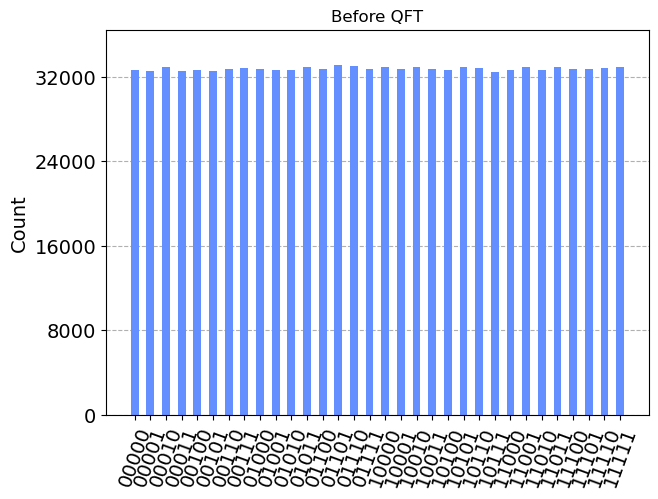
\includegraphics[scale=0.3]{code_snippets/qft1.png}
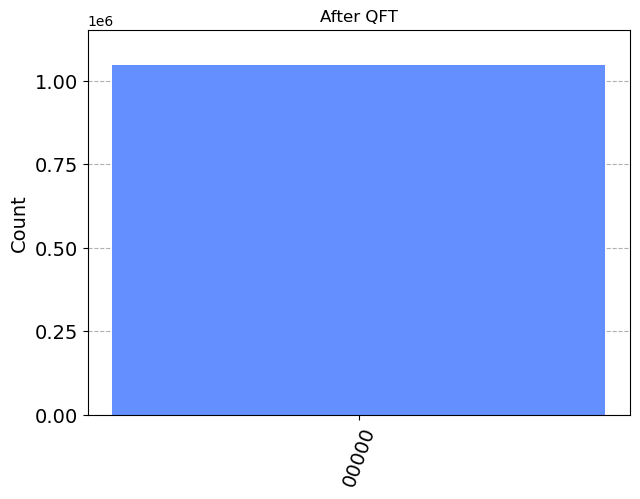
\includegraphics[scale=0.3]{code_snippets/qft2.png}



\caption{Basis states before and after a quantum Fourier transform}

\end{figure}











\subsubsection{Phase Estimation}

In simple terms, given an eigenstate $\lambda_{i}$ of a unitary $U$, phase estimation provides an estimate of the corresponding eigenvalue $e^{i\lambda_i}$. Phase estimation uses the quantum Fourier transform to estimate the phase kicked back by a unitary operation. A series of controlled versions of the unitary operation are performed on an input state. Figure \ref{fig:phase_estimation} shows an example with 4 control qubits. The control qubits are put in uniform superposition before applying the controlled operations.  More specifically, $j$ control qubits are used to apply the unitary $U^{2^{j}}$ controlled by the $j^{th}$ control qubit.

We know from phase kickbak that for $U = \sum_i e^{i \lambda_i} \lvert \lambda _i \rangle $, with any input $\lvert \psi \rangle = \sum_{k} c_k \lvert \lambda_i \rangle$.

We know that the work register will remain unchanged when the controlled unitaries are applied, even if the input $\lvert \psi \rangle$ is not an eigenstate of  $U = \sum_i e^{i \lambda_i} \lvert \lambda _i \rangle $, since we can decompose the input into the eigenbasis of U as  $\lvert \psi \rangle = \sum_{k} c_k \lvert \lambda_k \rangle$.

Denoting $c_j U^{2^{j}}$ as the unitary $U^{2^{j}}$ applied to the work register, controlled by the $j^{th}$ qubit, form the phase kickback result we have

\begin{multline}
\prod_{j=0}^{J-1} (c_j U^{2^{j}}) ( \frac{1}{2^{\frac{J-1}{2}}}( \lvert 0 \rangle + \lvert 1 \rangle )^{\otimes J-1} \lvert \psi \rangle)
\\
 =  \frac{1}{2^{\frac{J-1}{2}}} \bigotimes_{j=0}^{J-1} ( \lvert 0 \rangle + e^{i \lambda_i 2^{j}} \lvert 1 \rangle ) \lvert \psi \rangle
\\
 =  \frac{1}{2^{\frac{J-1}{2}}} \sum_{k=0}^{2^{J-1}-1}  ( \lvert 0 \rangle + e^{i k \lambda_i } \lvert 1 \rangle ) \lvert \psi \rangle
\\
\end{multline}

Comparing $product form equation$ with the product form of the quantum Fourier transform in \ref{eq:qft_product}, we can clearly see that performing the inverse quantum Fourier transform will give us

Using the phase kickbak result we have

clock and work register names


\begin{figure}[h]

\centering

\scalebox{0.7}{
\Qcircuit @C=1.0em @R=0.2em @!R { \\
	 	\nghost{{Clock\;Register}_{0} :  } & \lstick{{Clock\;Register}_{0} :  } & \gate{\mathrm{H}} & \qw & \qw & \qw & \ctrl{4} & \multigate{3}{\mathrm{IQFT}}_<<<{0} & \meter & \qw & \qw & \qw & \qw & \qw\\
	 	\nghost{{Clock\;Register}_{1} :  } & \lstick{{Clock\;Register}_{1} :  } & \gate{\mathrm{H}} & \qw & \qw & \ctrl{3} & \qw & \ghost{\mathrm{IQFT}}_<<<{1} & \qw & \meter & \qw & \qw & \qw & \qw\\
	 	\nghost{{Clock\;Register}_{2} :  } & \lstick{{Clock\;Register}_{2} :  } & \gate{\mathrm{H}} & \qw & \ctrl{2} & \qw & \qw & \ghost{\mathrm{IQFT}}_<<<{2} & \qw & \qw & \meter & \qw & \qw & \qw\\
	 	\nghost{{Clock\;Register}_{3} :  } & \lstick{{Clock\;Register}_{3} :  } & \gate{\mathrm{H}} & \ctrl{1} & \qw & \qw & \qw & \ghost{\mathrm{IQFT}}_<<<{3} & \qw & \qw & \qw & \meter & \qw & \qw\\
	 	\nghost{{Work\;Register} :  } & \lstick{{Work\;Register} :  } & \qw & \gate{\mathrm{U\string^1}} & \gate{\mathrm{U\string^2}} & \gate{\mathrm{U\string^4}} & \gate{\mathrm{U\string^8}} & \qw & \qw & \qw & \qw & \qw & \qw & \qw\\
	 	\nghost{\mathrm{{Output} :  }} & \lstick{\mathrm{{Output} :  }} & \lstick{/_{_{4}}} \cw & \cw & \cw & \cw & \cw & \cw & \dstick{_{_{\hspace{0.0em}0}}} \cw \ar @{<=} [-5,0] & \dstick{_{_{\hspace{0.0em}1}}} \cw \ar @{<=} [-4,0] & \dstick{_{_{\hspace{0.0em}2}}} \cw \ar @{<=} [-3,0] & \dstick{_{_{\hspace{0.0em}3}}} \cw \ar @{<=} [-2,0] & \cw & \cw\\
\\ }}



\caption{Circuit for quantum phase estimation}

\label{fig:phase_estimation}

\end{figure}

The phase estimation algorithm requires multiple ancilla qubits. A more efficient implementation is the iterative phase estimation algorithm, which requires a single qubit to perform phase estimation.


\subsubsection{Amplitude Amplification}

Amplitude Amplification is used to boost the success probability of a desired ouput. The procedure is proven to be optimal and provides a quadratic inprovement in success probability.

Consider an arbitrary quantum state $\lvert \psi \rangle$ and a projective measurement 

Consider a quantum algorithm  $\mathcal{A} $ s.t. 
\begin{equation}
\mathcal{A} \lvert 0 \rangle^{\otimes n} = \sqrt{p} \lvert \psi_{good} \rangle + \sqrt{1-p} \lvert \psi_{bad} \rangle
\end{equation}
 where $ \lvert \psi_{good} \rangle $ is the desired output with success probability $p$. The amplitude amplification procedure will boost the success probability to $O(1)$ using $O( \sqrt{g} )$ applicatoins of $\mathcal{A}$.

More specifically, this is achieved using $O(\sqrt{p})$ applications of the operator $\mathcal{Q}$:

\begin{equation}
\mathcal{Q} = \mathcal{A} \mathcal{S}_0 \mathcal{A}^\dagger \mathcal{S}_{good}
\end{equation}

where 

\begin{equation}
\mathcal{S}_0  = \mathbb{I} - 2 \lvert 0 \rangle ^{\otimes n} \langle 0 \rvert  ^{\otimes n}
\end{equation}

is a reflection operation about the state $\lvert 0 \rangle ^{\otimes n}$ and 

\begin{equation}
\mathcal{S}_0  = \mathbb{I} - 2 \lvert \psi_{good} \rangle \langle \psi_{good} \rvert  
\end{equation}

is an oracle for reflection about the state $ \lvert \psi_{good} \rangle $. Intuitively these operations can also be interpreted as 'marking' the states $\lvert 0 \rangle ^{\otimes n}$. Note that the operations are in fact Householder reflectors.

The overall circuit is provided in Figure \ref{fig:amplitude_amplification}


\begin{figure}[h]

\centering

\scalebox{1.0}{
\Qcircuit @C=1.0em @R=0.2em @!R { \\
	 	\nghost{{\lvert \psi\ \rangle ^ {\otimes n}} :  } & \lstick{{\lvert \psi\ \rangle ^ {\otimes n}} :  } & \gate{\mathcal{A}} & \gate{\mathcal{Q}^{O(\sqrt{g})}} & \qw & \qw\\
\\ }}

\caption{Circuit for amplitude amplification}

\label{fig:amplitude_amplification}

\end{figure}


Grover's search algorithm is a special case of amplitude amplification, which can search for an entry in an unstructured database of $N$ entries in $O(\sqrt{N})$ time compared to $O(N)$ time needed classically.





\subsubsection{Hamiltonian Simulation}

Hamiltonian simulation is simply applying the operation $U \approx e^{-iHt}$ to a quantum state. Since $H$ is a Hermitian matrix, $U$ is unitary. The Hamiltonian simulation subroutine is important for simulating quantum systems like quantum chemistry problems and is also used in the HHL quantum linear system algorithm. It encodes the evolution of a quantum state according to the Schrodinger equation:

\begin{equation}
\frac{d}{dt} \lvert \Psi(t) \rangle = -i H \lvert \Psi(t) \rangle
\end{equation}

where the Planck constant has been absorbed into the Hamiltonian $H$, which has the solution

\begin{equation}
\lvert \Psi (t) \rangle = e^{-iHt} \lvert \Psi(0) \rangle
\end{equation}

Various methods exist for Hamiltonian simulation, the most important ones being Trotter-Suzuki product formulas, Taylor series approximations using linear combinations of unitaries, and quantum signal processing.

Suzuki-Trotter, or Trotter formulas use the Baker-Campbel-Hausdorff formula to approximate

\begin{equation}
e^{-i \mathbf{H} t} = e^{ -i \sum_{j=0}^{k}\mathbf{H}_j t } = (e^{ -i \sum_{j=0}^{k}\mathbf{H}_j t / r})^r \approx   (\prod_{j=0}^{k} e^{-i \mathbf{H}_j t / r })^r + O(k^2 t^2 / r)
\end{equation}


Higher order Trotter formulas can be constructed to further reduce the error. Although the error in Trotter formulas does not scale well, they have the advantage of not requiring additional (ancilla) qubits. As an example, the second order Trotter formula is

\begin{equation}
e^{-i \mathbf{H} t} = e^{ -i \sum_{j=0}^{k}\mathbf{H}_j t } = (e^{ -i \sum_{j=0}^{k}\mathbf{H}_j t / r})^r \approx   (\prod_{j=0}^{k} e^{-i \mathbf{H}_j t / 2r }\prod_{j=k}^{0} e^{-i \mathbf{H}_j t / 2r })^r + O(k^3 t^3 / r^2)
\end{equation}


The Taylor series approximation using a linear combination of unitaries uses a slightly different approach by decomposing $H$ as a sum of unitaries $H_l$

\begin{equation}
U = e^{-i \mathbf{H} t}  = ( e^{-i \mathbf{H} t/r} )^r = (U_r)^r
\end{equation}

\begin{equation}
U_r  \approx \hat U_r = \sum_{k=0}^{K} \sum_{l_1,...,l_k=1}^{L} \frac{(-it/r)^k}{k!} \alpha_{l_1} ... \alpha_{l_k} \mathbf{H}_{l_1} ... \mathbf{H}_{l_k} 
\label{eqn:taylor}
\end{equation}

A choice of $K = O(\frac{\log(r/\epsilon)}{\log \log (r/\epsilon)})$ leads to a precision $\lVert U - (\hat U_r)^r \rVert _2 \leq \epsilon$, an exponential improvement over Trotter simulations. However, to apply the sum in Equation \ref{eqn:taylor} the linear combination of unitaries method is used, which requires ancilla qubits and has a non-zero probability of success.

The quantum signal processing method uses a complex polynomial approximation of $e^{-i \mathbf{H} t}$ using the quantum signal processing protocol. This involves applying the quantum signal processing circuit 

\begin{equation}
U_\Phi (H) = e^{-i\phi_0 Z} \prod_{j=1}^{d} [O(H) e^{-i\phi_j Z}]
\end{equation}

where $\phi_j$ are quantum signal processing angles independent of the particular problem and $O(H)$ is a block encoding of a Hamiltonian. The error decreases exponentially with the number of phase angles used. The phase angles may be calculated using QSPPACK. This method is also referred to as Qubitization.


We provide here as an example a Hamiltonian simulation of  $\mathbf{H} = X + Z$ using the first- and second- order Trotter method for for various $t$, for varying numbers of Trotter steps, with the error plots shown in \ref{fig:trotter}:

\lstinputlisting[language=Python]{code_snippets/trotter.py}

\begin{figure}[!h]
\centering

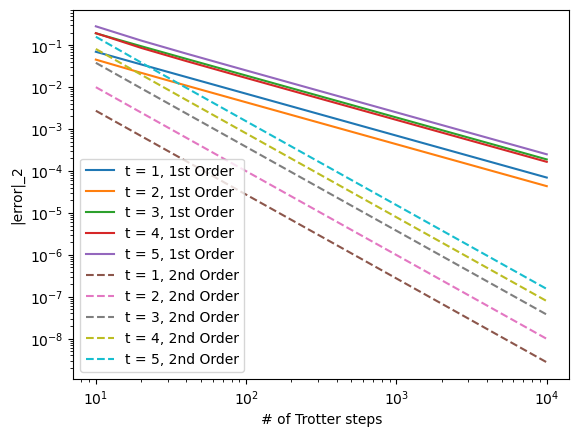
\includegraphics[scale=0.75]{code_snippets/trotter_output.png}

\label{fig:trotter}
\caption{Output of Trotter Code}

\end{figure}



\subsection{Quantum Linear System Algorithms}

Quantum linear system algorithms are perhaps the most lucrative area of quantum computing for scientific and engineering computation.

The quantum linear system algorithms solve the quantum linear system problem. The quantum linear system problem is slightly different from the classical linear system problem and can formally be stated as

Given a quantum state $\lvert \mathbf{b} \rangle$, prepare a state $\lvert \mathbf{x} \rangle$ with precision $\epsilon$ s.t. $ \mathbf{Ax=b} $.

Due to normalization of quantum states, the quantum state $\lvert \mathbf{x} \rangle$ is proportional to the solution $\mathbf{x}$. Furthermore, unlike classical solutions, the quantum state encodes the solution instead of the entire solution being available classically.

A plethora of quantum linear system algorithms exist, of which the most notable are the HHL algorithm, the LCU algorithm, and the QSP algorithm.

The HHL algorithm is the first proposed algorithm and it uses Hamiltonian simulation to apply controlled versions of $e^{-iAt}$ on the state $\lvert b \rangle$. Since $A$ and $e^{-iAt}$ share the same eigenvectors, the eigenvalues of $e^{-iAt}$ are kicked back to the control qubits. Using the quantum Fourier transform, eigenvalues are encoded in the amplitudes of the control qubits. Finally, a controlled rotation on an ancilla is used to invert the eigenvalues. The computation is then reversed to disentangle the registers, and the ancilla is measured. Measurement of the ancilla in the desired state indicates successful solution.

The LCU algorithm works by using a  Chebyshev polynomial approximation $P(x) \approx 1/x$ over the interval $x \in I_P : [-1,-1/\kappa]\cup[1/\kappa,1]$, where $\kappa$ is the condition number of the system. The matrix polynomial approximation $P(A)$ is applied to the state $\lvert b \rangle$ to obtain the approximate solution $A^{-1}b \approx P(A) b$. Given a desired precision $\lVert P(x) - \frac{1}{x} \rVert _{\max x \in I_P} \leq \epsilon$, $P(x)$ is a polynomial of degree $O(\kappa \log{\frac{1}{\epsilon}})$. However, applicatoin of a linear combination of unitaries has an additional overhead in the form of ancilla qubits. 

The QSP method circumvents the issue of ancilla qubits by applying $P(A)$ as a product of unitary operations rather than a sum. This entails finding a sequence of angles $\mathbf{\phi}$, the quantum signal processing angles, corresponding to the desired polynomial and a block encoding of the matrix.

For positive-definite systems it is possible to achieve the $\sqrt{\kappa}$ scaling of classical solvers. We first define the alternative polynomial approximation $Q(y) \approx y = \frac{1}{1-x}$ over the interval $y \in I_Q : [-1,1/\kappa]$, and define $B = I - \eta A$ where $\eta$ is chosen s.t. $\lVert B \rVert \leq 1$. Given a desired precision $\lVert Q(x) - \frac{1}{x} \rVert _{\max x \in I_Q} \leq \epsilon$, $Q(x)$ is a polynomial of degree $O(\sqrt{\kappa} \log{\frac{1}{\epsilon}})$. The matrix polynomial approximation $Q(B)$ is then applied to the quantum state $\lvert b \rangle$.

We provide as an example a linear solver using quantum signal processing.


\subsection{Quantum Eigenvalue Problem}

Time-independent Schrodinger equation, or the ground state problem.


\subsection{Quantum Algorithms for Systems of Ordinary Differential Equations}

Quantum algorithms for systems of ordinary differential equations may broadly be classified as homogeneous, inhomogeneous, linear, nonlinear, and variational. Of course, higher order differential equations can trivially be transformed into a system of first order ordinary differential equations.

The solution of homogenous linear differential equations can simply be stated as a Hamiltonian simulation problem, since the time-dependent Schrodinger equation for a closed quantum system is a first order linear differential equation. There are several drawbacks to using this method, and we turn out attention instead to the more general homogeneous linear differential equation case.


The first efficient quantum algorithm for inhomogeneous linear differential equations was proposed by {Berry 2014}. The method utilizes high-order linear multistep methods to approximate the time evolution given an initial condition. This is achieved by encoding the sequence of linear operations as back-substitution in a larger linear system, and solving the larger linear system. This method achieved a sub-optimal scaling of $t^2$, and an improved version was presented by {Lloyd}?. This method was soon superseded by {Berry 2017}, which instead of using the linear multistep methods directly applies the time-discretized time propagation operator $e^{Ah}$, where $h$ is the time-step, using a Taylor series approximation of $e^{Ah}$. This method achieves exponential advantage with exponentially improved dependence on precision, and scales linearly with time as $t$. However, recent work has shown that positive-definite systems of linear equations can be solved with $\sqrt{\kappa}$ complexity, an improvement over the earlier bound of $\kappa$. Since the linear systems formed in {Berry 2014, 2017} are positive-definite, we state here an improved version of their algorithm with a quadratic dependence in time.


The first quantum algorithm for differential equations was proposed by {Leyton}. {Leyton}'s algorithm proposed solving a nonlinear system of ordinary differential equations using the Euler method, and achieved an overall scaling of {}. The algorithm requires preparation of multiple copies of a quantum state to effect nonlinear transformations of amplitude encoded states. Using the block encoding technique nonlinear transformations of the singular values of a matrix operator $A$ can be performed. However, nonlinear transformations of the amplitudes of a state as an input to a nonlinear function is not possible using this technique. {Leyton} requires multiple copies of a state to create polynomial terms of the amplitudes. This leads to an exponential cost in simulation time.






Several algorithms have been proposed for linear, nonlinear, homogeneous, and non-homogeneous systems of ordinary differential equations. For nonlinear systems algorithms using Koopman and Carleman linearization have been proposed. Exponential speedups have theorized for the linear systems of ordinary differential equations. Since the non-homogeneous system of ordinary differential equations is of general interest, we provide here an overview of the algorithm.

We also note that higher order systems of ordinary differential equations can easily be converted to linear systems, therefore this algorithm holds for the general case of linear ordinary differential equations.

The algorithm involves solving a large linear system that encodes the evolution of an ordinary differential equation at all time steps, intermediate and final. The encoding is performed using a Taylor series approximation of the general matrix exponential, which propagates the solution in time.




\subsection{Quantum Algorithms for Partial Differential Equations}


\subsection{Variational Algorithms and Quantum Machine Learning}





\end{document}

